We perform the analysis on a dataset corresponding to $1.1\pm0.1\ifb$ integrated luminosity. 
In this section we document the results obtained after the $\zz$ preselection and the 
final mass-dependent $\hzz$ selections using cut-based approach. 

\subsection{Results after the $\zz$ preselection}
The dilepton $p_T$ distribution is shown in Figure \ref{fig:zpt_zzpresel} after a very loose
cut on the minimum of \met and track \met to be above 20 GeV to take into account data
skimming requirements.  We select events with a dilepton $p_T$ above 40 GeV.
The distribution of the minimum of \met and track \met is shown after the dilepton $p_T$
cut in Figure \ref{fig:minmet_zzpresel}.  The $M_T$ distributions are shown in
Figure \ref{fig:mt_zzpresel} after requiring the minimum of \met and track \met to be 
greater than 50 GeV.  This is referred to as the \zz preselection.

Table~\ref{tab:zzselection_all} shows the number of events observed in
data, comparing to the expected background contribution at the \zz
preselection level. The background estimation was discussed at Section~\ref{sec:backgrounds}.

%%%%%%%%
\begin{table}[!ht]
\begin{center}
\begin{tabular} {c|c|c|cccccc}
\hline
  & data & all bkg. & $\dyll$ & $\ZZ$ & $\WZ$ & $WW$ & $\ttbar+tW$ & $\Wjets$  \\
\hline
\multicolumn{9}{c} {0 Jet Bin} \\
\hline
 $\mu\mu$ &  39 & $43.4\pm0.9$ & $8.2\pm0.1$ & $14.5\pm0.3$ & $7.1\pm0.3$ & $11.6\pm0.4$ & $2.1\pm0.7$ & $0.0$ \\
 $ee$     &  31 & $31.7\pm0.8$ & $8.2\pm0.1$ & $9.7\pm0.2$  & $4.0\pm0.2$ & $7.5\pm0.3$ & $1.0\pm0.3$ & $1.3\pm0.6$ \\
\hline
\multicolumn{9}{c} {1 Jet Bin} \\
\hline
 $\mu\mu$ &  21 & $22.6\pm0.8$ & $8.8\pm0.1$ & $3.7\pm0.1$ & $3.7\pm0.2$ &  $3.3\pm0.2$ & $3.1\pm0.7$ & $0.0$  \\
 $ee$     &  18 & $19.6\pm0.9$ & $8.8\pm0.1$ & $2.6\pm0.1$ & $2.5\pm0.2$ & $2.2\pm0.2$ & $3.6\pm0.8$ & $0.0$ \\
\hline
\end{tabular}
\caption{Expected number of signal and background events from the data-driven methods for an 
  integrated luminosity of \intlumi  after applying the $\ZZ$ selection requirements. 
Only statistical uncertaities are reported. }
   \label{tab:zzselection_all}
  \end{center}
\end{table}
%%%%%%%%

%%%%%%%%
\begin{figure}[!hbtp]
\begin{center}
\label{fig:zpt_zzpresel}
\subfigure[0-Jet]{\label{subfig:zpt_0j}
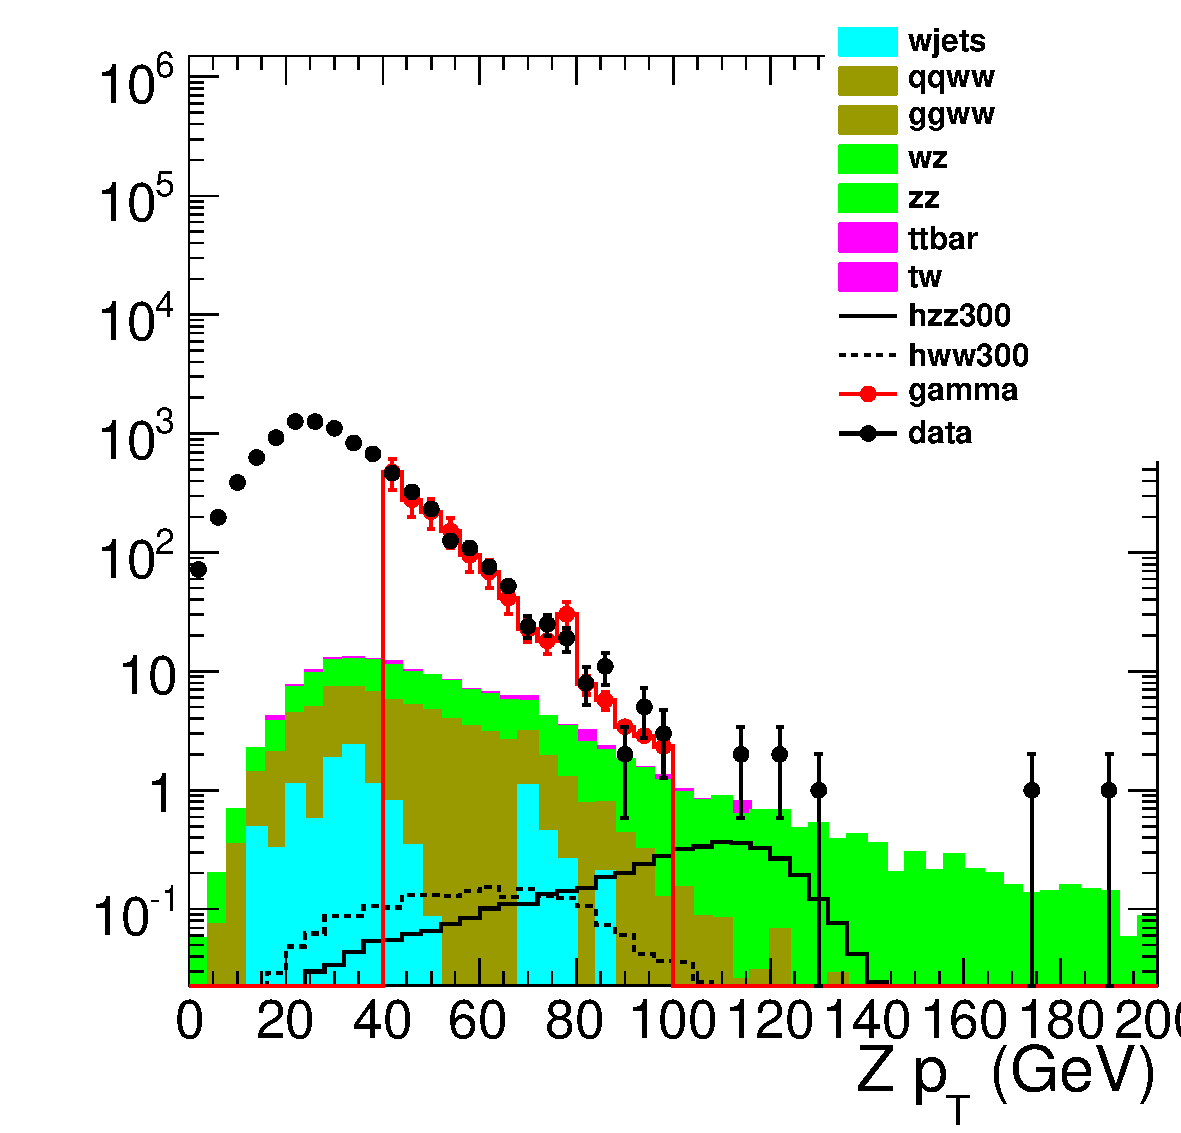
\includegraphics[width=.3\textwidth]{figures/presel_hzz300_zpt_0j_log.pdf}}
\subfigure[1-Jet]{\label{subfig:zpt_1j}
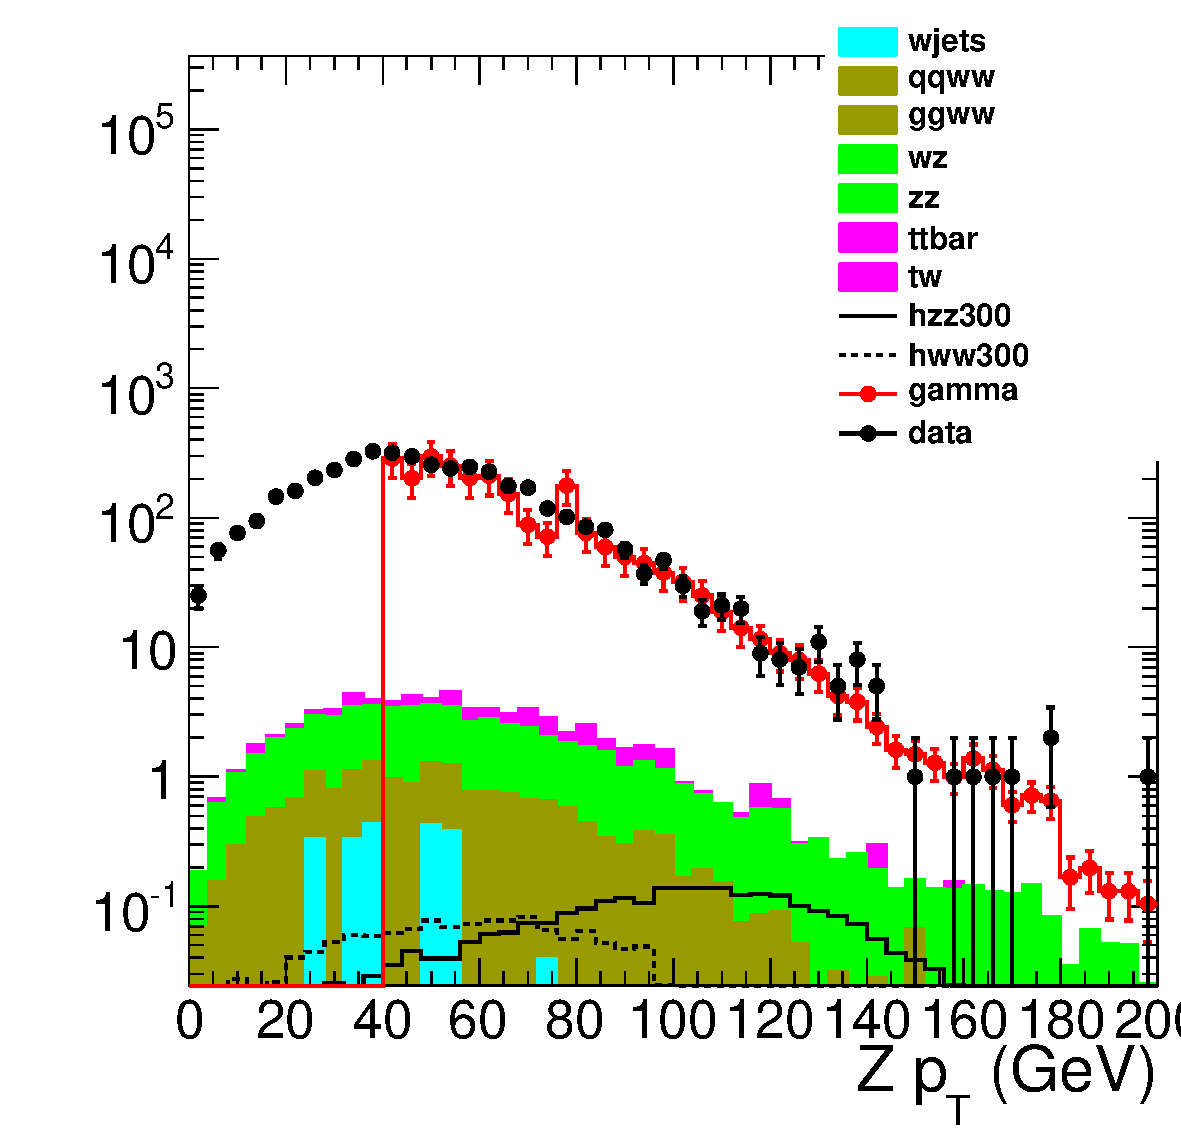
\includegraphics[width=.3\textwidth]{figures/presel_hzz300_zpt_1j_log.pdf}}
\subfigure[$\geq$2 Jets]{\label{subfig:zpt_2j}
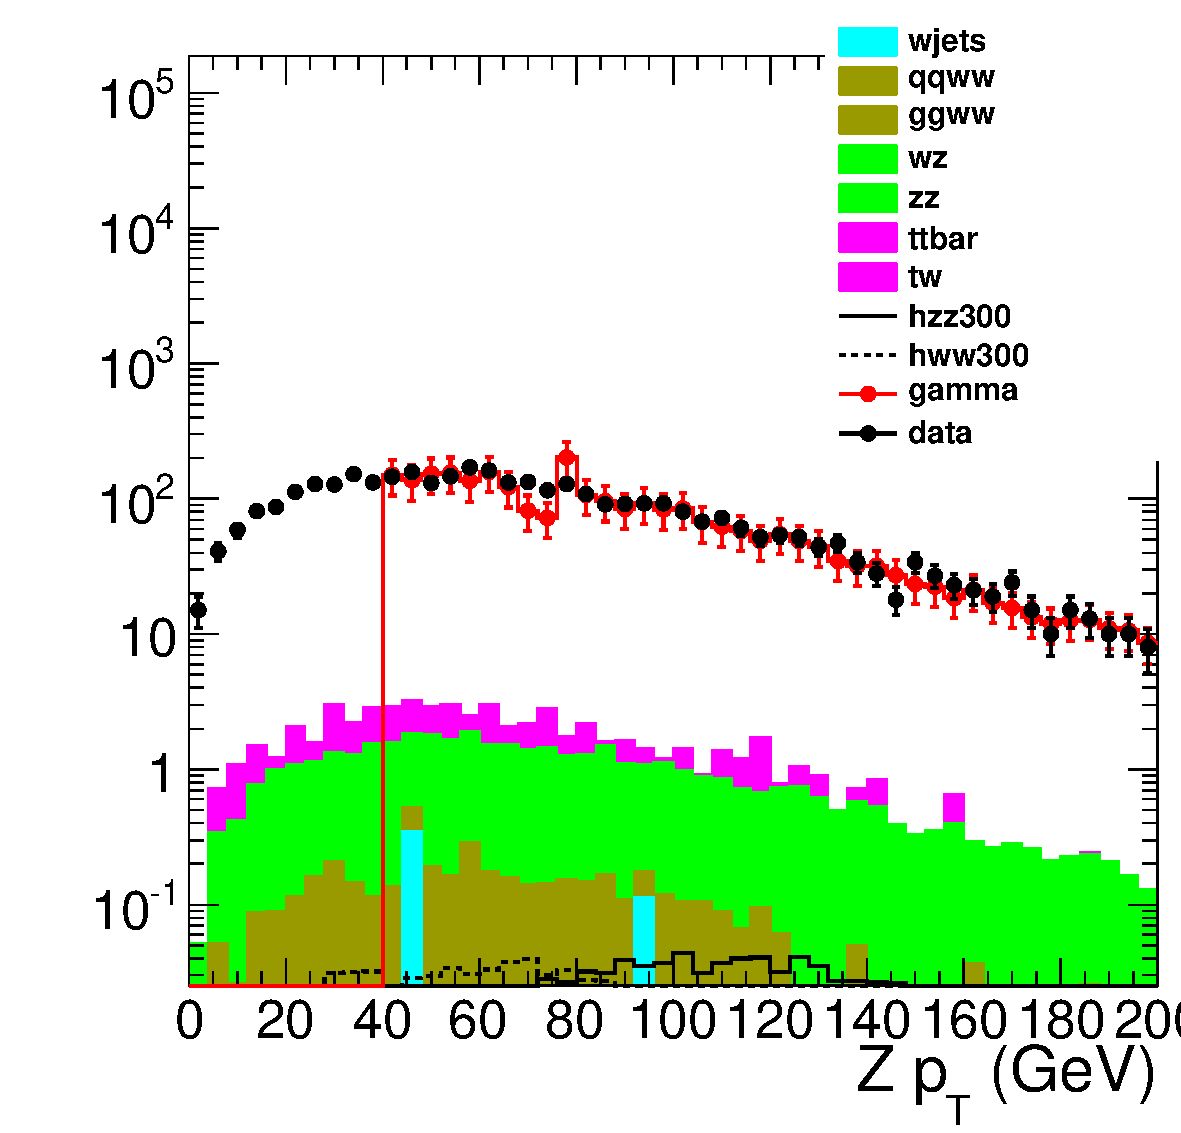
\includegraphics[width=.3\textwidth]{figures/presel_hzz300_zpt_2j_log.pdf}}
\caption{Dilepton $p_T$ distribution after the $\ZZ$ preselection observed in data corresponding to $1092\pm7$~\ipb data in 0-Jet~\subref{subfig:zpt_0j}, 1-Jet~\subref{subfig:zpt_1j}
and 2-Jet~\subref{subfig:zpt_2j} bins, compared to the expected from simulation for signal and background.
The MC backgrounds are scaled as appropriate and the photon+jets estimate of the Z+jets background is added to the stack.}
\end{center}
\end{figure}
%%%%%%%%

%%%%%%%%
\begin{figure}[!hbtp]
\begin{center}
\label{fig:minmet_zzpresel}
\subfigure[0-Jet]{\label{subfig:minmet_0j}
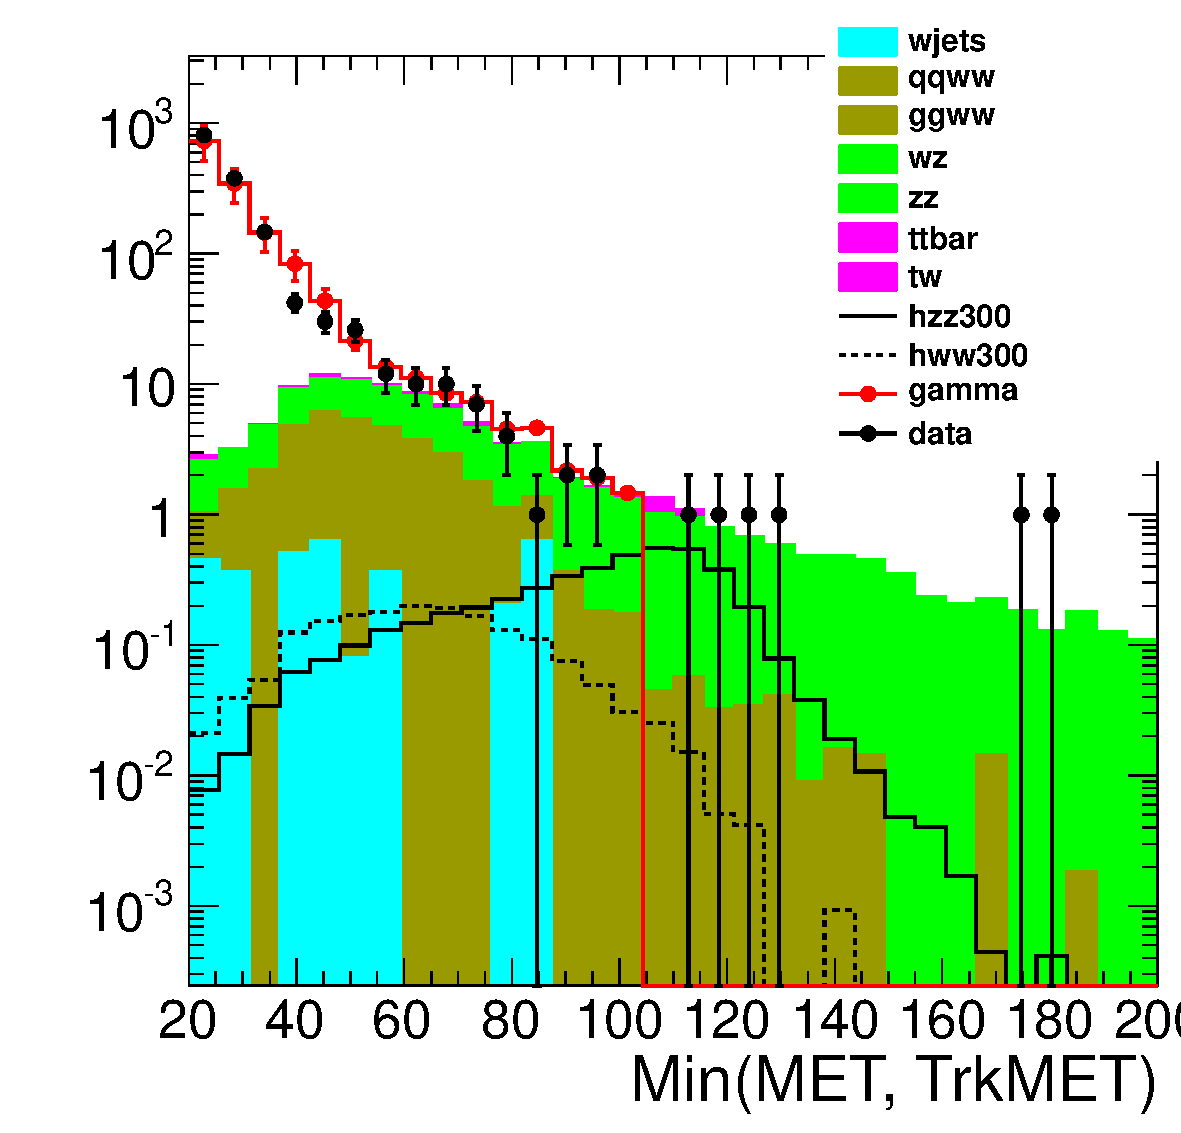
\includegraphics[width=.3\textwidth]{figures/presel_hzz300_minmet_0j_log.pdf}}
\subfigure[1-Jet]{\label{subfig:minmet_1j}
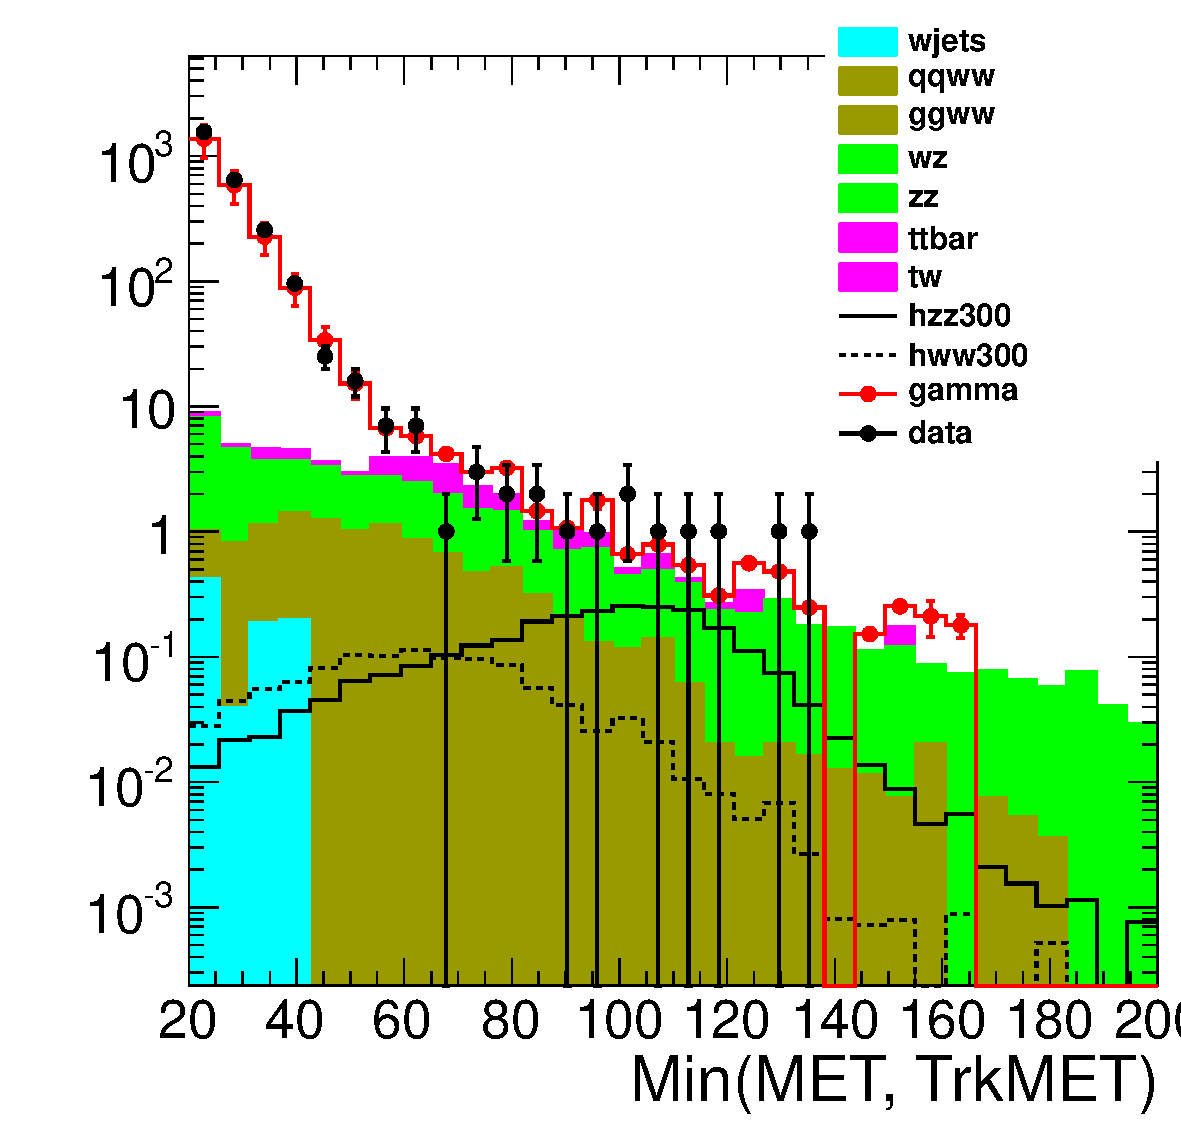
\includegraphics[width=.3\textwidth]{figures/presel_hzz300_minmet_1j_log.pdf}}
\subfigure[$\geq$2 Jets]{\label{subfig:minmet_2j}
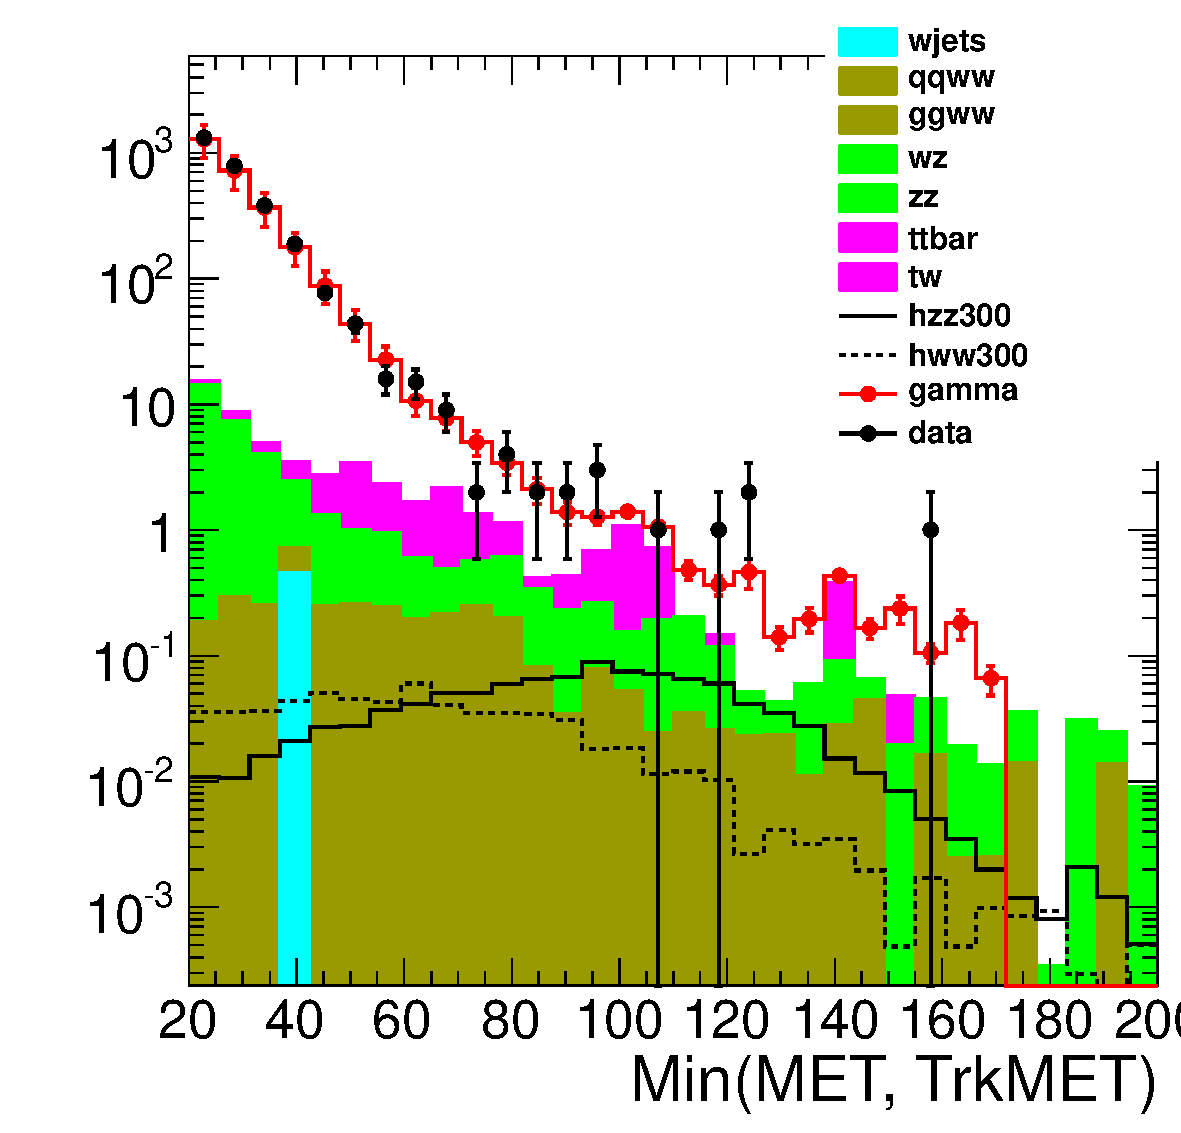
\includegraphics[width=.3\textwidth]{figures/presel_hzz300_minmet_2j_log.pdf}}
\caption{Min-MET distribution after the $\ZZ$ preselection observed in data corresponding to $1092\pm7$~\ipb data in 0-Jet~\subref{subfig:minmet_0j}, 1-Jet~\subref{subfig:minmet_1j} 
and 2-Jet~\subref{subfig:minmet_2j} bins, compared to the expected from simulation for signal and background. 
The MC backgrounds are scaled as appropriate and the photon+jets estimate of the Z+jets background is added to the stack.}
\end{center}
\end{figure}
%%%%%%%%


%%%%%%%%
\begin{figure}[!hbtp]
\begin{center}
\label{fig:mt_zzpresel}
\subfigure[0-Jet]{\label{subfig:mt_0j}
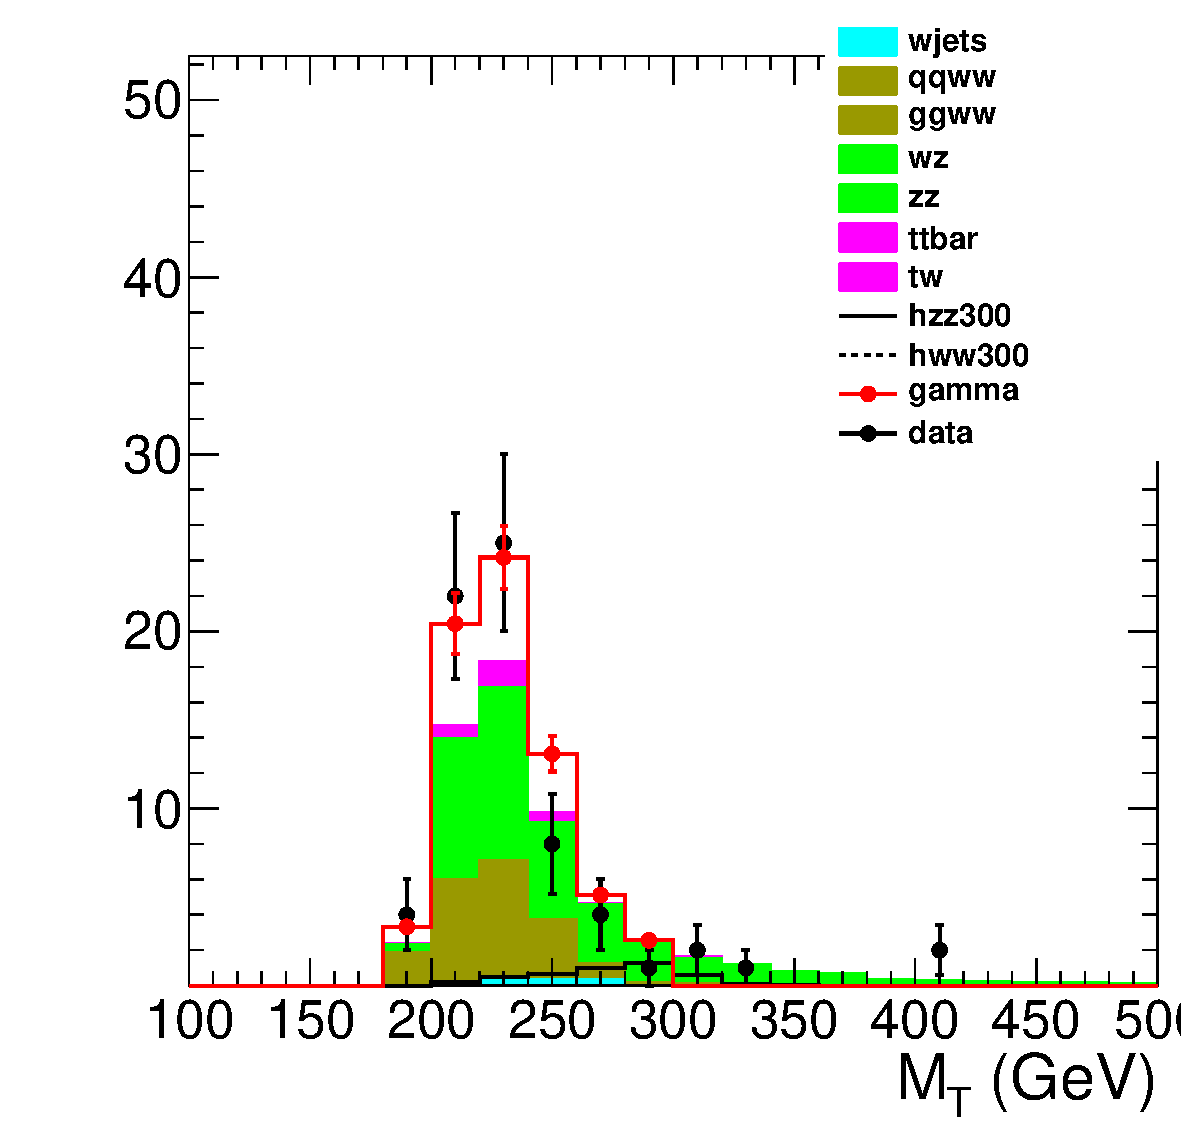
\includegraphics[width=.3\textwidth]{figures/presel_hzz300_mt_0j.pdf}}
\subfigure[1-Jet]{\label{subfig:mt_1j}
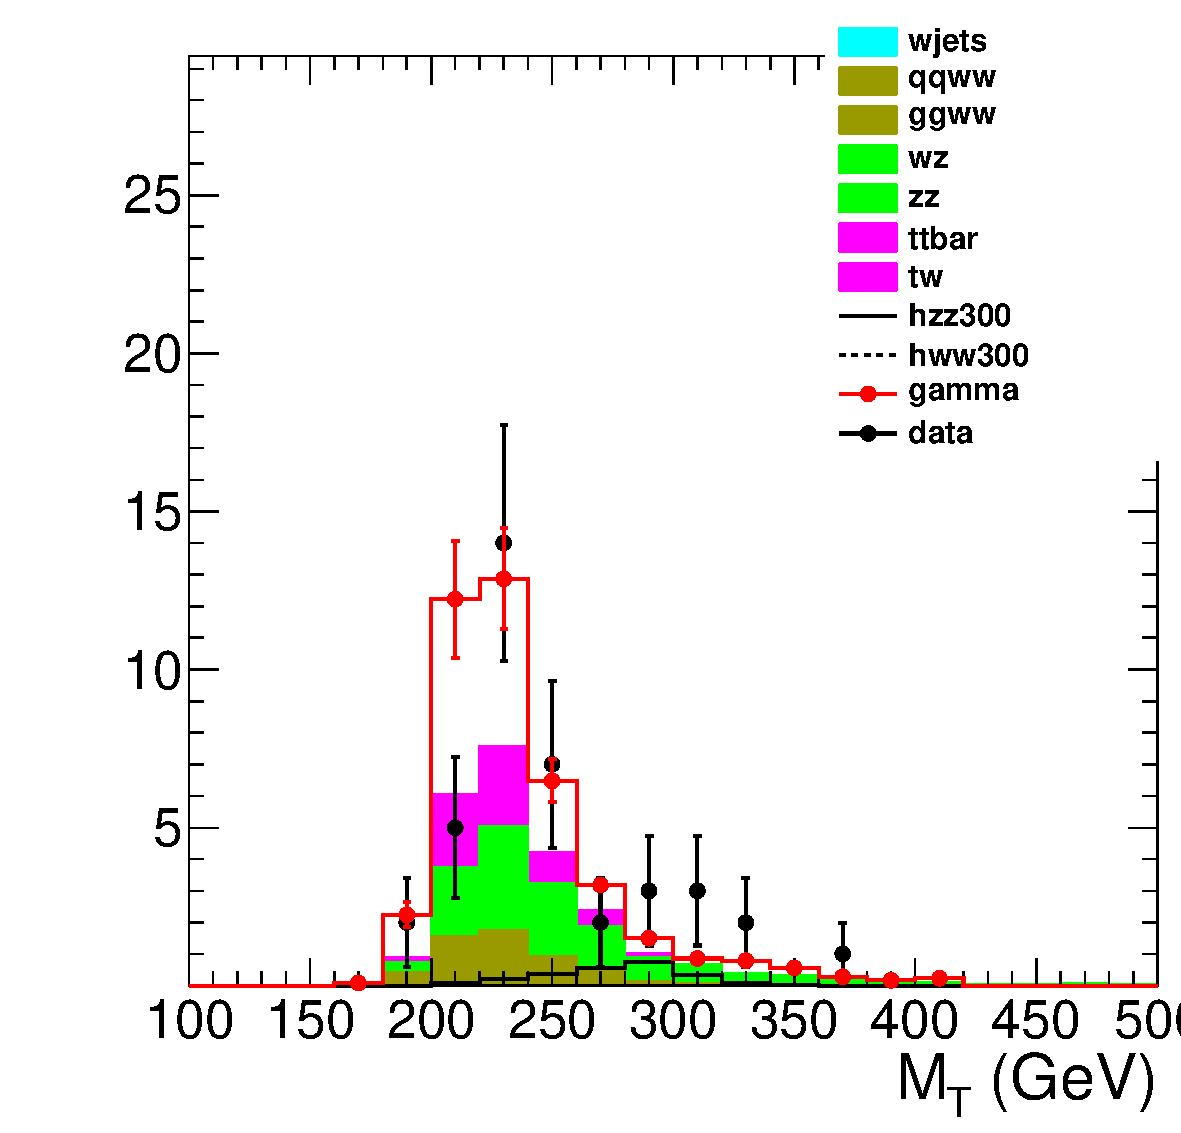
\includegraphics[width=.3\textwidth]{figures/presel_hzz300_mt_1j.pdf}}
\subfigure[$\geq$2 Jets]{\label{subfig:mt_2j}
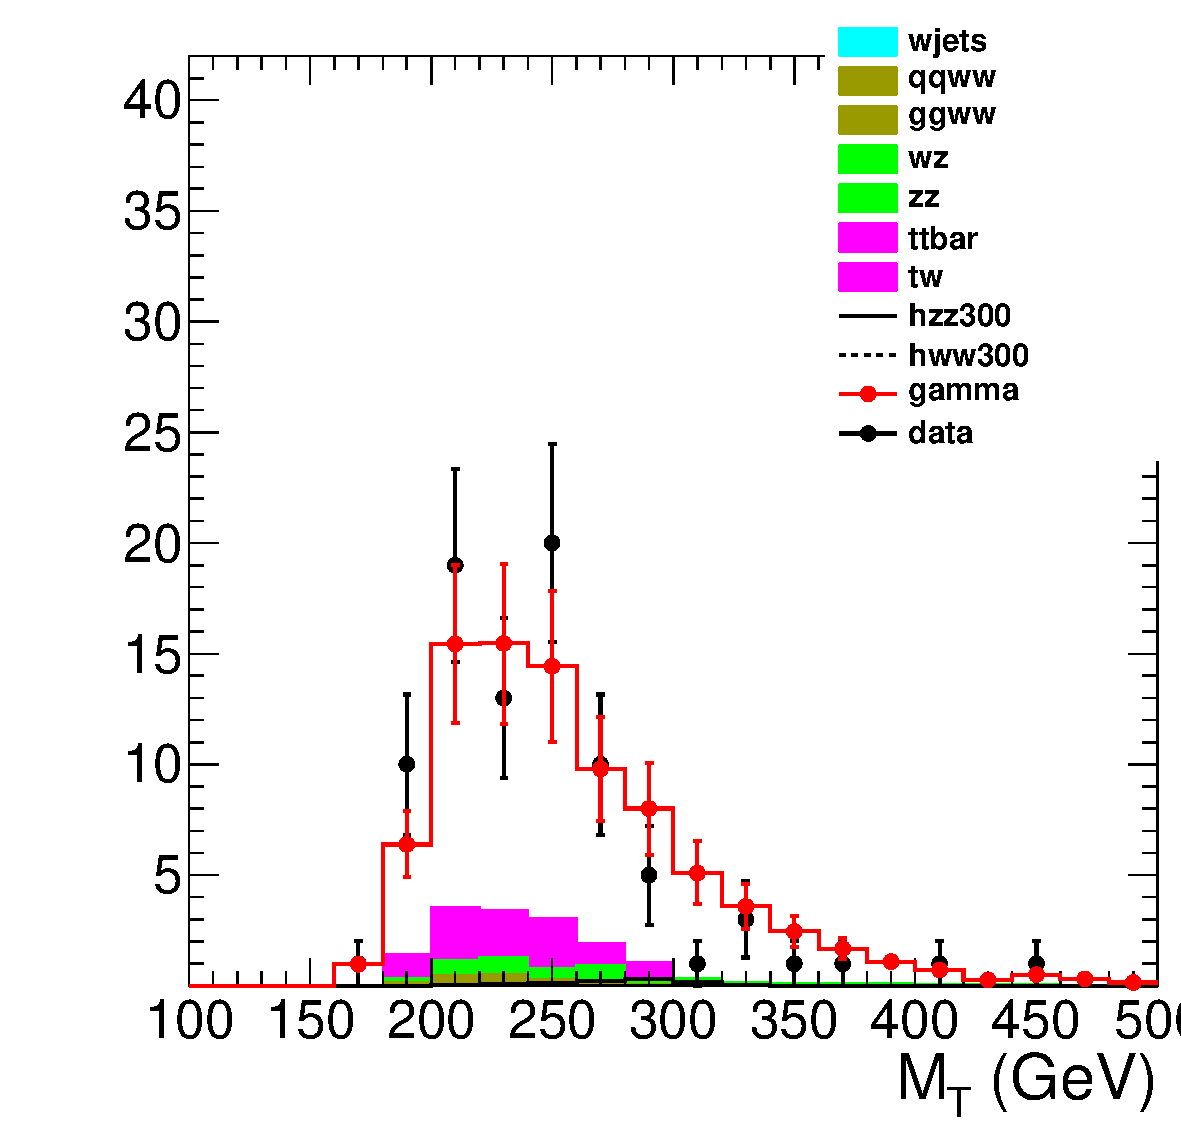
\includegraphics[width=.3\textwidth]{figures/presel_hzz300_mt_2j.pdf}}
\caption{Transverse mass $m_T$ distribution after the $\ZZ$ preselection observed in data corresponding to $1092\pm7$~\ipb data in 0-Jet~\subref{subfig:mt_0j}, 1-Jet~\subref{subfig:mt_1j} 
and 2-Jet~\subref{subfig:mt_2j} bins, compared to the expected from simulation for signal and background. 
The MC backgrounds are scaled as appropriate and the photon+jets estimate of the Z+jets background is added to the stack.}
\end{center}
\end{figure}
%%%%%%%%

\clearpage

\subsection{Results after the $\hzz$ final selection}
The Higgs boson mass dependent signal selections are described in Section \ref{sec:signal_selection}. 
In this section we summarise the results obtained in zero and one jet final states only. 
The reasons are as follows,
%%%%%%%%%
\begin{itemize}
\item The 2-Jet bin final state is sensitive to the vector-boson-fusion production mode. 
Currently we do not have the MC samples for the $\hzz$ produced in VBF mode.
\item The final sensistivity is driven by the zero and one jet bins as the background contribution especially from the 
Drell-Yan processes are very much shown in Table~\ref{tab:zzselection_all}.
\end{itemize}
%%%%%%%%%
We plan to include the two-jet bin final states for the next iteration of the results. 

After applying these signal selections, which differ only from the \zz preselection
in terms of the \met and $M_T$ cuts, the resulting $M_T$ distributions are shown
in Figures \ref{fig:mt_hzz250}, \ref{fig:mt_hzz300} and \ref{fig:mt_hzz400} respectively.
Tables~\ref{tab:yield_hzz250}-\ref{tab:yield_hzz400} show the equivalent data yields
and background expectations.
A more detailed break down of the event yields can be found in ~\ref{app:yield1fbdetail}.


%%%%%%%%
%\begin{table}[!ht]
%\begin{center}
%\begin{tabular} {c|c|c|c|ccccc}
%\hline
%  & data & $HZZ$(200) & all bkg. & $\dyll$ & $\ZZ$ & $\WZ$ & $WW$ & $\ttbar+tW$ \\
%\hline
%\multicolumn{9}{c} {0 Jet Bin} \\
%\hline
% $\mu\mu$ &  12 & $0.12\pm0.01$ & $13.9\pm0.4$ & $3.34\pm0.04$ & $3.1\pm0.1$ & $2.1\pm0.2$ & $4.8\pm0.2$ & $0.5\pm0.3$ \\
% $ee$     &  14 & $0.07\pm0.01$ & $9.9\pm0.3$  & $3.34\pm0.04$ & $2.0\pm0.1$ & $1.2\pm0.1$ & $3.1\pm0.2$ & $0.2\pm0.2$ \\
%\hline
%\multicolumn{9}{c} {1 Jet Bin} \\
%\hline
% $\mu\mu$ &  0 & $0.02\pm0.00$ & $0.34\pm0.10$ & $0.12\pm0.01$ & $0.02\pm0.01$ & $0.01\pm0.01$ & $0.07\pm0.03$ & $0.13\pm0.09$ \\
% $ee$     &  0 & $0.01\pm0.00$ & $0.20\pm0.03$ & $0.12\pm0.01$ & $0.01\pm0.01$ & $0.02\pm0.01$ & $0.05\pm0.02$ & $0.0$ \\
%\hline
%\end{tabular}
%\caption{Expected number of signal and background events from the data-driven methods for an 
%  integrated luminosity of \intlumi  after applying the $\hzz$ ($m_H=200\GeVcc$) selection requirements. 
%Only statistical uncertaities are reported. The $\Wjets$ background is neglible thus omitted in the table.}
%   \label{tab:yield_hzz200}
%  \end{center}
%\end{table}
%%%%%%%%


%%%%%%%%
\begin{table}[!ht]
\begin{center}
\begin{tabular} {c|c|c|c|ccccc}
\hline
  & data & $HZZ$(250) & all bkg. & $\dyll$ & $\ZZ$ & $\WZ$ & $WW$ & $\ttbar+tW$ \\
\hline
\multicolumn{9}{c} {0 Jet Bin} \\
\hline
 $\mu\mu$ &  20 & $2.12\pm0.04$ & $16.7\pm0.7$ & $3.4\pm0.1$ & $5.3\pm0.2$ & $2.7\pm0.2$ & $4.0\pm0.2$ & $1.4\pm0.0.6$ \\
 $ee$     &  7 & $1.57\pm0.03$ & $12.7\pm0.6$ & $3.4\pm0.1$ & $3.5\pm0.1$ & $1.6\pm0.1$ & $2.9\pm0.2$ & $0.5\pm0.2$ \\
\hline
\multicolumn{9}{c} {1 Jet Bin} \\
\hline
 $\mu\mu$ &  5 & $1.02\pm0.02$ & $9.1\pm0.6$ & $2.38\pm0.02$ & $1.4\pm0.1$ & $1.8\pm0.2$ & $1.7\pm0.1$ & $1.8\pm0.5$ \\
 $ee$     &  8 & $0.70\pm0.02$ & $8.6\pm0.8$ & $2.38\pm0.02$ & $1.1\pm0.1$ & $1.1\pm0.1$ & $1.2\pm0.1$ & $2.9\pm0.8$ \\
\hline
\end{tabular}
\caption{Expected number of signal and background events from the data-driven methods for an 
  integrated luminosity of \intlumi  after applying the $\hzz$ ($m_H=250\GeVcc$) selection requirements. 
Only statistical uncertaities are reported. The $\Wjets$ background is neglible thus omitted in the table.}
   \label{tab:yield_hzz250}
  \end{center}
\end{table}
%%%%%%%%
%%%%%%%%
\begin{table}[!ht]
\begin{center}
\begin{tabular} {c|c|c|c|ccccc}
\hline
  & data & $HZZ$(300) & all bkg. & $\dyll$ & $\ZZ$ & $\WZ$ & $WW$ & $\ttbar+tW$ \\
\hline
\multicolumn{9}{c} {0 Jet Bin} \\
\hline
 $\mu\mu$ &  3 & $1.67\pm0.03$ & $5.4\pm0.2$ & $0.26\pm0.03$ & $2.9\pm0.1$ & $1.3\pm0.1$ & $0.8\pm0.1$ & $0.09\pm0.0.05$ \\
 $ee$     &  4 & $1.18\pm0.02$ & $3.6\pm0.2$ & $0.26\pm0.03$ & $2.2\pm0.1$ & $0.6\pm0.1$ & $0.4\pm0.1$ & $0.14\pm0.14$ \\
\hline
\multicolumn{9}{c} {1 Jet Bin} \\
\hline
 $\mu\mu$ &  1 & $0.60\pm0.01$ & $1.3\pm0.2$ & $0.16\pm0.01$ & $0.47\pm0.05$ & $0.26\pm0.06$ & $0.14\pm0.04$ & $0.25\pm0.22$ \\
 $ee$     &  2 & $0.43\pm0.01$ & $0.9\pm0.1$ & $0.16\pm0.01$ & $0.34\pm0.04$ & $0.15\pm0.04$ & $0.13\pm0.03$ & $0.08\pm0.08$ \\
\hline
\end{tabular}
\caption{Expected number of signal and background events from the data-driven methods for an  
integrated luminosity of \intlumi  after applying the $\hzz$ ($m_H=300\GeVcc$) selection requirements. 
Only statistical uncertaities are reported. The $\Wjets$ background is neglible thus omitted in the table.}
   \label{tab:yield_hzz300}
  \end{center}
\end{table}
%%%%%%%%
%%%%%%%%
\begin{table}[!ht]
\begin{center}
\begin{tabular} {c|c|c|c|ccccc}
\hline
  & data & $HZZ$(400) & all bkg. & $\dyll$ & $\ZZ$ & $\WZ$ & $WW$ & $\ttbar+tW$ \\
\hline
\multicolumn{9}{c} {0 Jet Bin} \\
\hline
 $\mu\mu$ &  1 & $1.29\pm0.02$ & $2.3\pm0.1$ & $0.0$ & $1.7\pm0.1$ & $0.55\pm0.08$ & $0$ & $0$ \\
 $ee$     &  2 & $0.94\pm0.02$ & $1.4\pm0.1$ & $0.0$ & $1.1\pm0.1$ & $0.25\pm0.06$ & $0$ & $0$ \\
\hline
\multicolumn{9}{c} {1 Jet Bin} \\
\hline
 $\mu\mu$ &  2 & $0.97\pm0.02$ & $1.5\pm0.1$ & $0.43\pm0.05$ & $0.68\pm0.06$ & $0.37\pm0.07$ & $0.05\pm0.02$ & $0$ \\
 $ee$     &  3 & $0.70\pm0.01$ & $1.1\pm0.1$ & $0.43\pm0.05$ & $0.46\pm0.05$ & $0.21\pm0.05$ & $0.04\pm0.01$ & $0$ \\
\hline
\end{tabular}
\caption{Expected number of signal and background events from the data-driven methods for an 
integrated luminosity of \intlumi  after applying the $\hzz$ ($m_H=400\GeVcc$) selection requirements. 
Only statistical uncertaities are reported. The $\Wjets$ background is neglible thus omitted in the table.}
   \label{tab:yield_hzz400}
  \end{center}
\end{table}
%%%%%%%%




%%%%%%%%
\begin{figure}[!hbtp]
\begin{center}
\label{fig:mt_hzz250}
\subfigure[0-Jet]{\label{subfig:mt_0j}
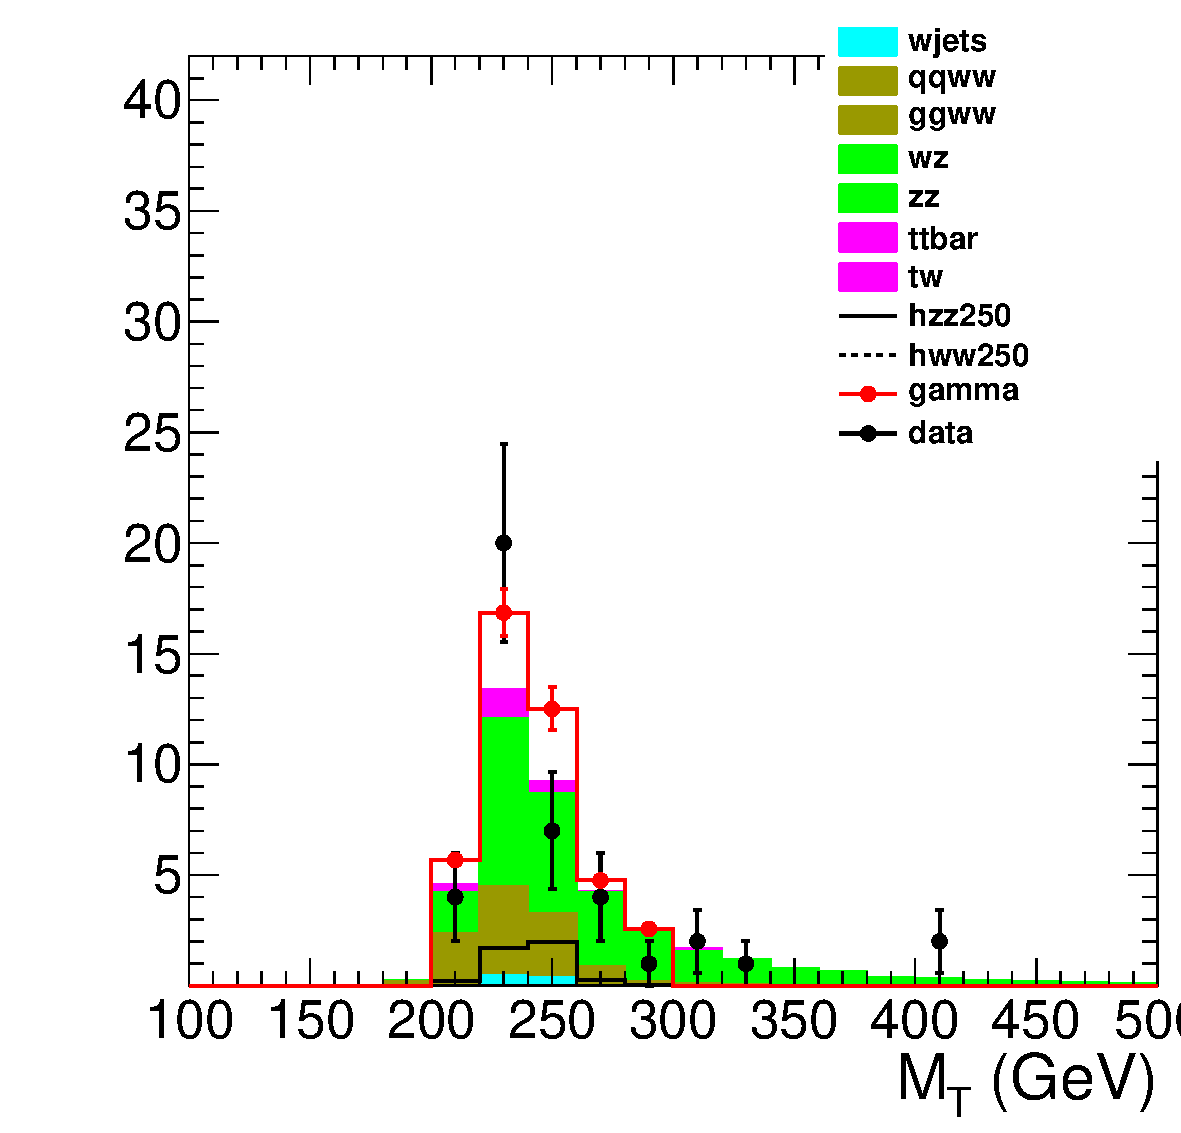
\includegraphics[width=.3\textwidth]{figures/hzz250_mt_0j.pdf}}
\subfigure[1-Jet]{\label{subfig:mt_1j}
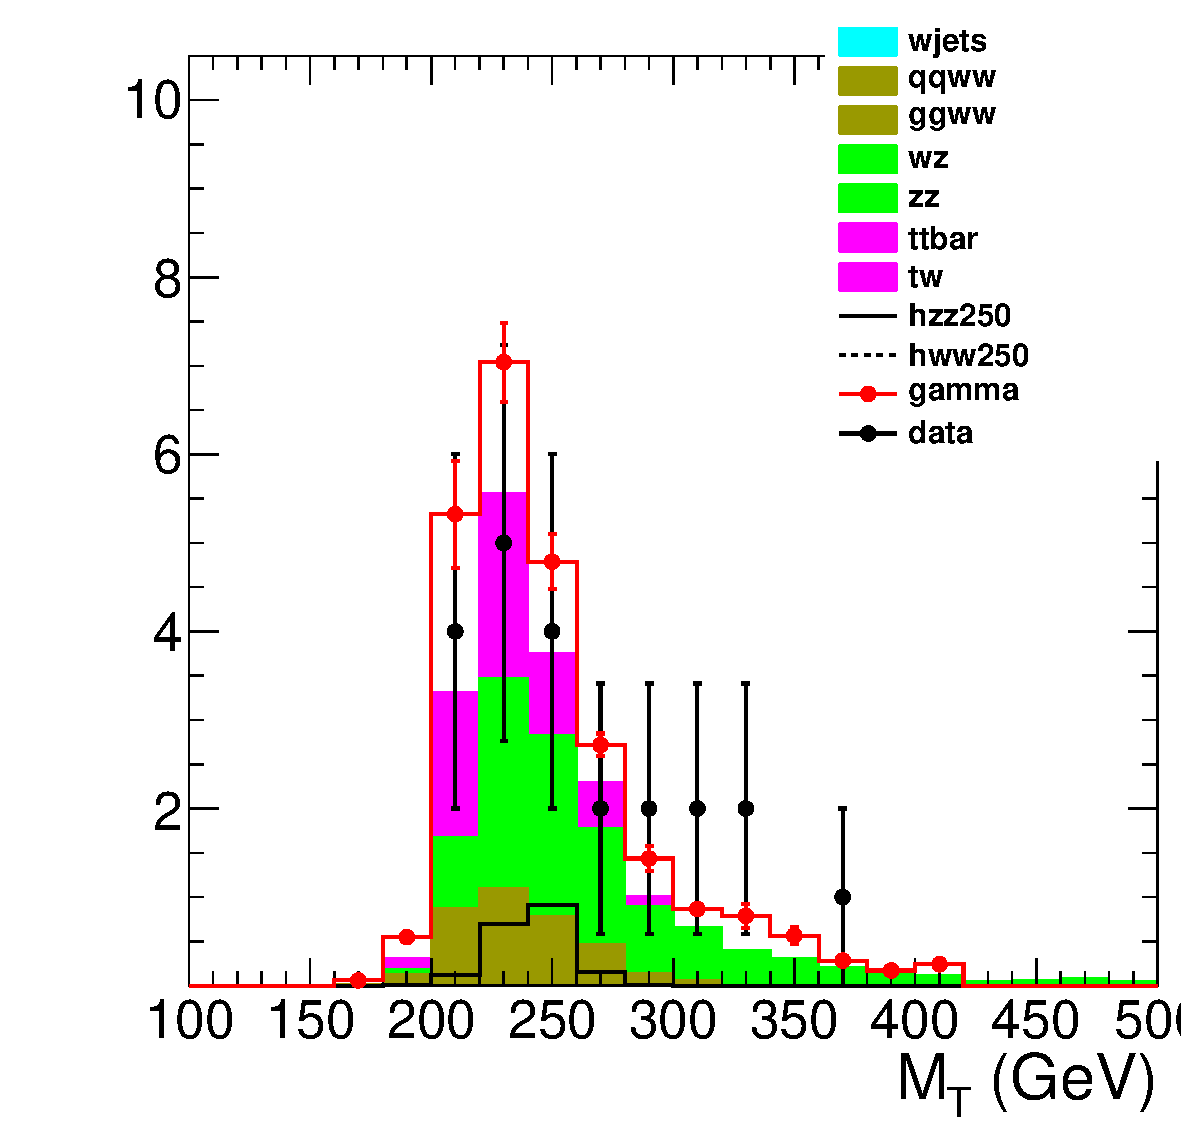
\includegraphics[width=.3\textwidth]{figures/hzz250_mt_1j.pdf}}
\caption{Transverse mass $m_T$ distribution after the full $\hzz$ ($m_H = 250\GeVcc$) selection observed in 
data corresponding to $1092\pm7$~\ipb data in 0-Jet~\subref{subfig:mt_0j} and 1-Jet~\subref{subfig:mt_1j}
bins compared to the expected from simulation for signal and background. 
The MC backgrounds are scaled as appropriate and the photon+jets estimate of the Z+jets background is added to the stack.}
\end{center}
\end{figure}
%%%%%%%%

%%%%%%%%
\begin{figure}[!hbtp]
\begin{center}
\label{fig:mt_hzz300}
\subfigure[0-Jet]{\label{subfig:mt_0j}
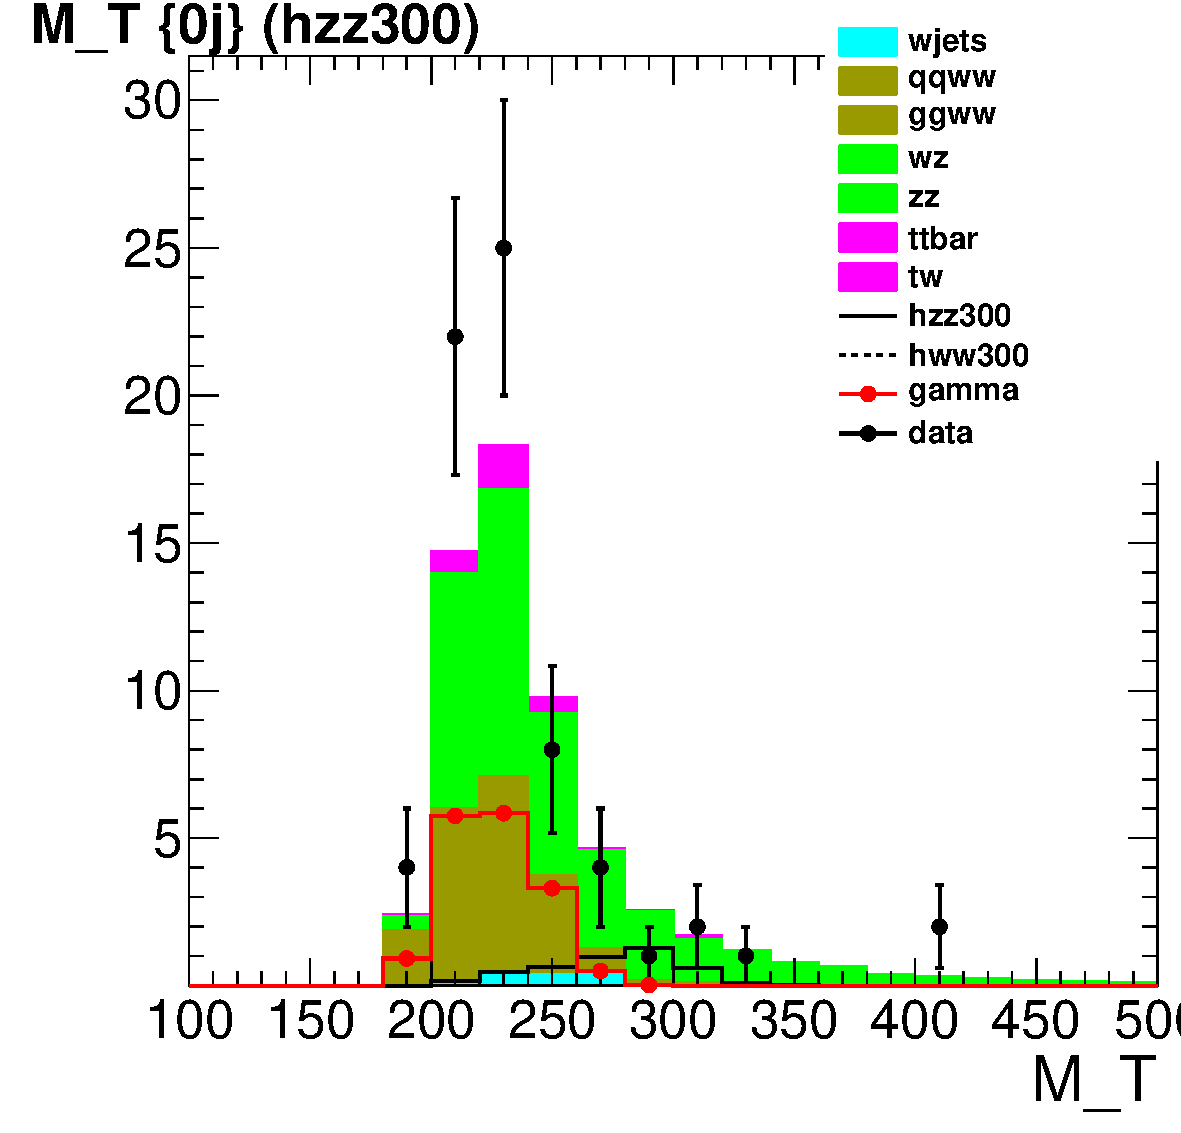
\includegraphics[width=.3\textwidth]{figures/hzz300_mt_0j.pdf}}
\subfigure[1-Jet]{\label{subfig:mt_1j}
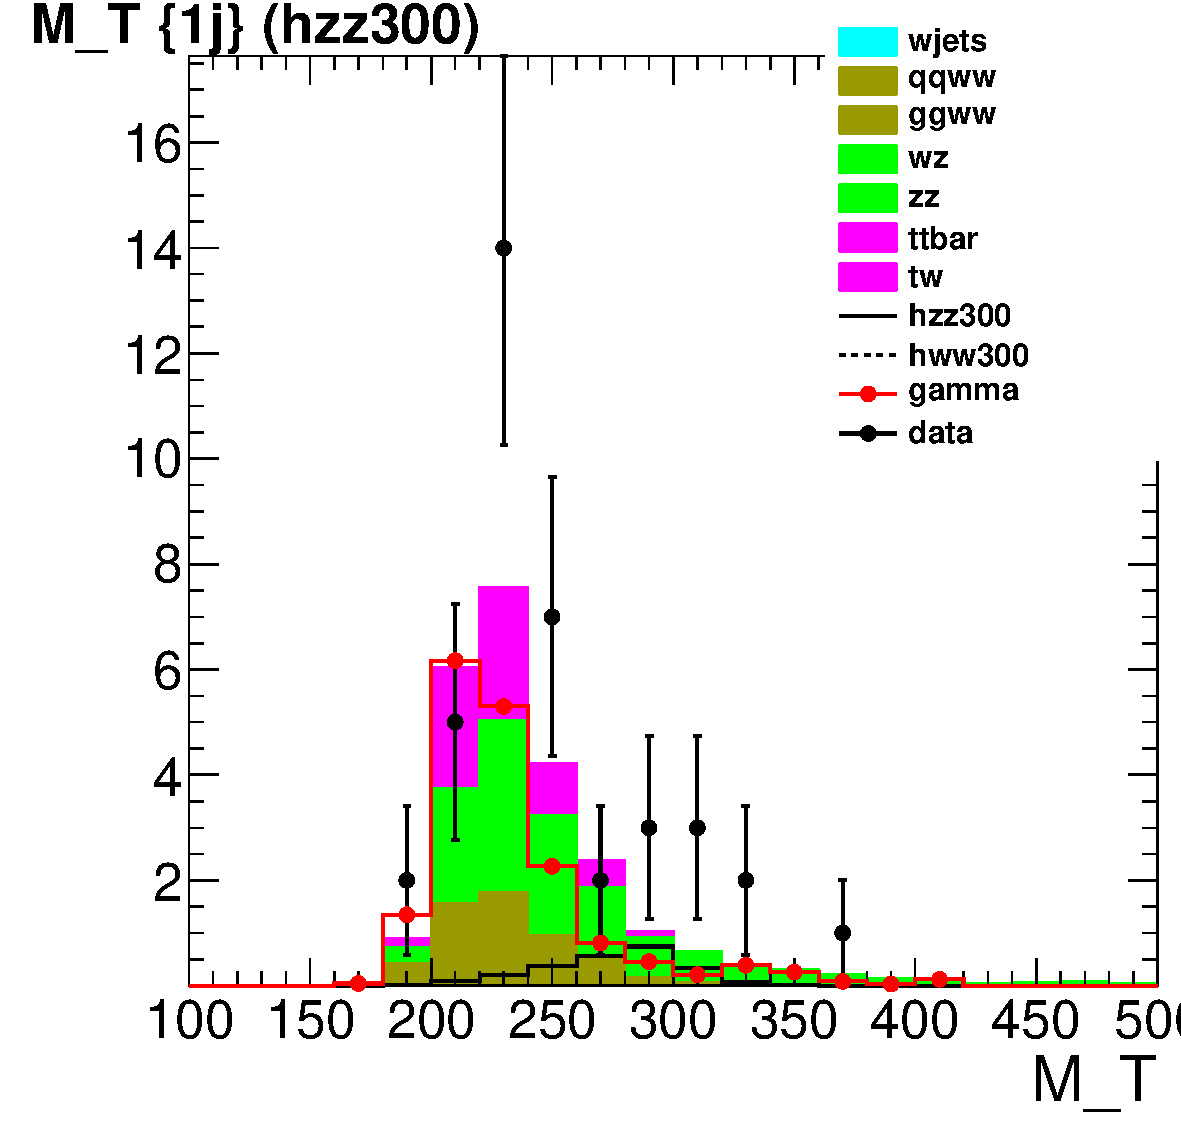
\includegraphics[width=.3\textwidth]{figures/hzz300_mt_1j.pdf}}
\caption{Transverse mass $m_T$ distribution after the full $\hzz$ ($m_H = 300\GeVcc$) selection observed in
data corresponding to $1092\pm7$~\ipb data in 0-Jet~\subref{subfig:mt_0j} and 1-Jet~\subref{subfig:mt_1j}
bins compared to the expected from simulation for signal and background. 
The MC backgrounds are scaled as appropriate and the photon+jets estimate of the Z+jets background is added to the stack.}
\end{center}
\end{figure}
%%%%%%%%

%%%%%%%%
\begin{figure}[!hbtp]
\begin{center}
\label{fig:mt_hzz400}
\subfigure[0-Jet]{\label{subfig:mt_0j}
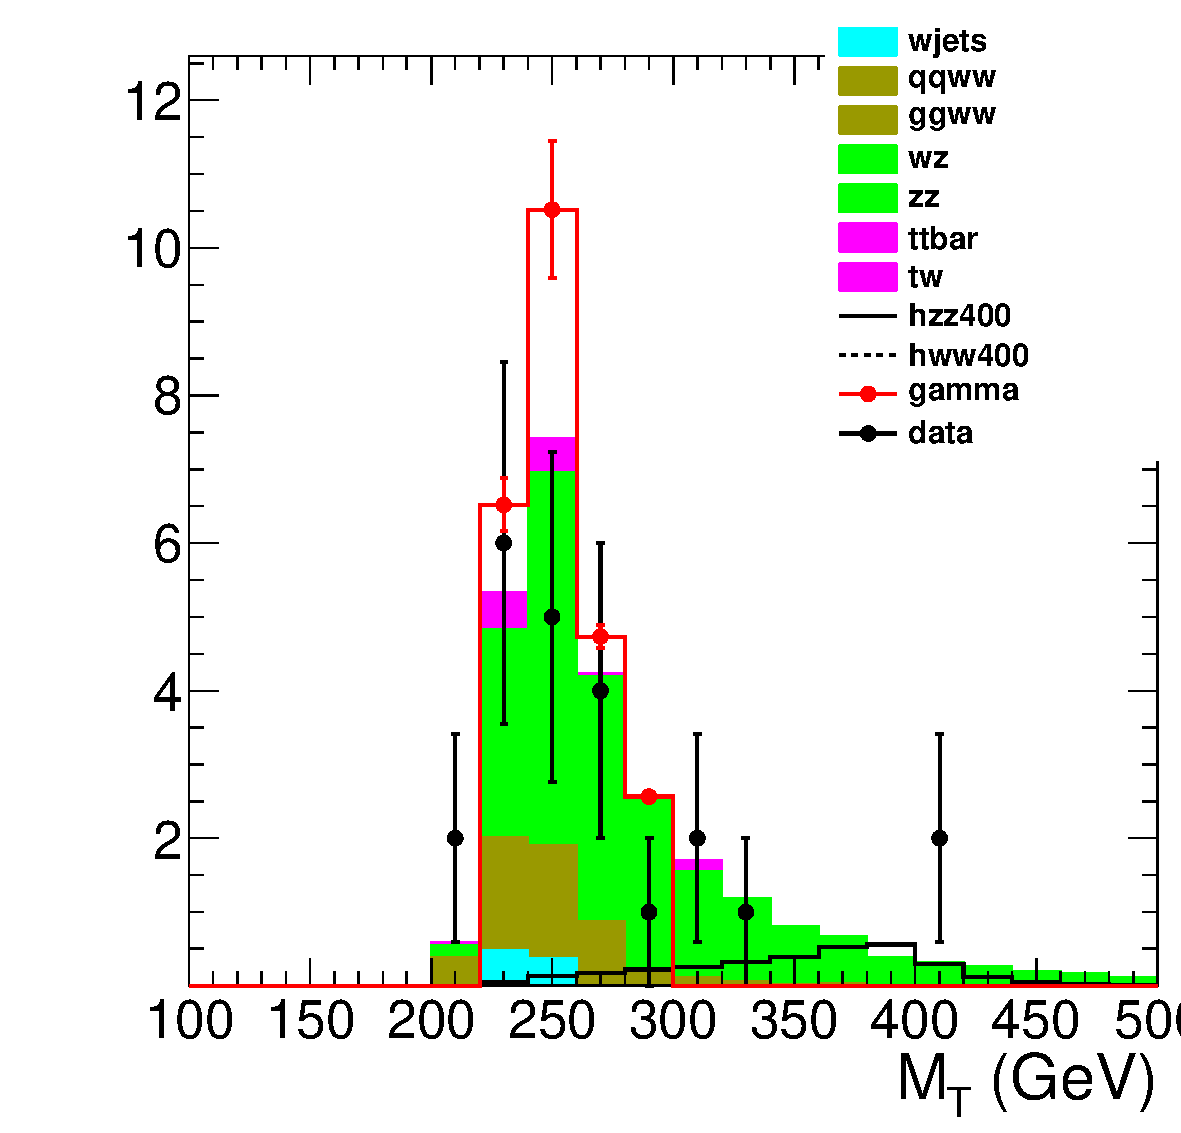
\includegraphics[width=.3\textwidth]{figures/hzz400_mt_0j.pdf}}
\subfigure[1-Jet]{\label{subfig:mt_1j}
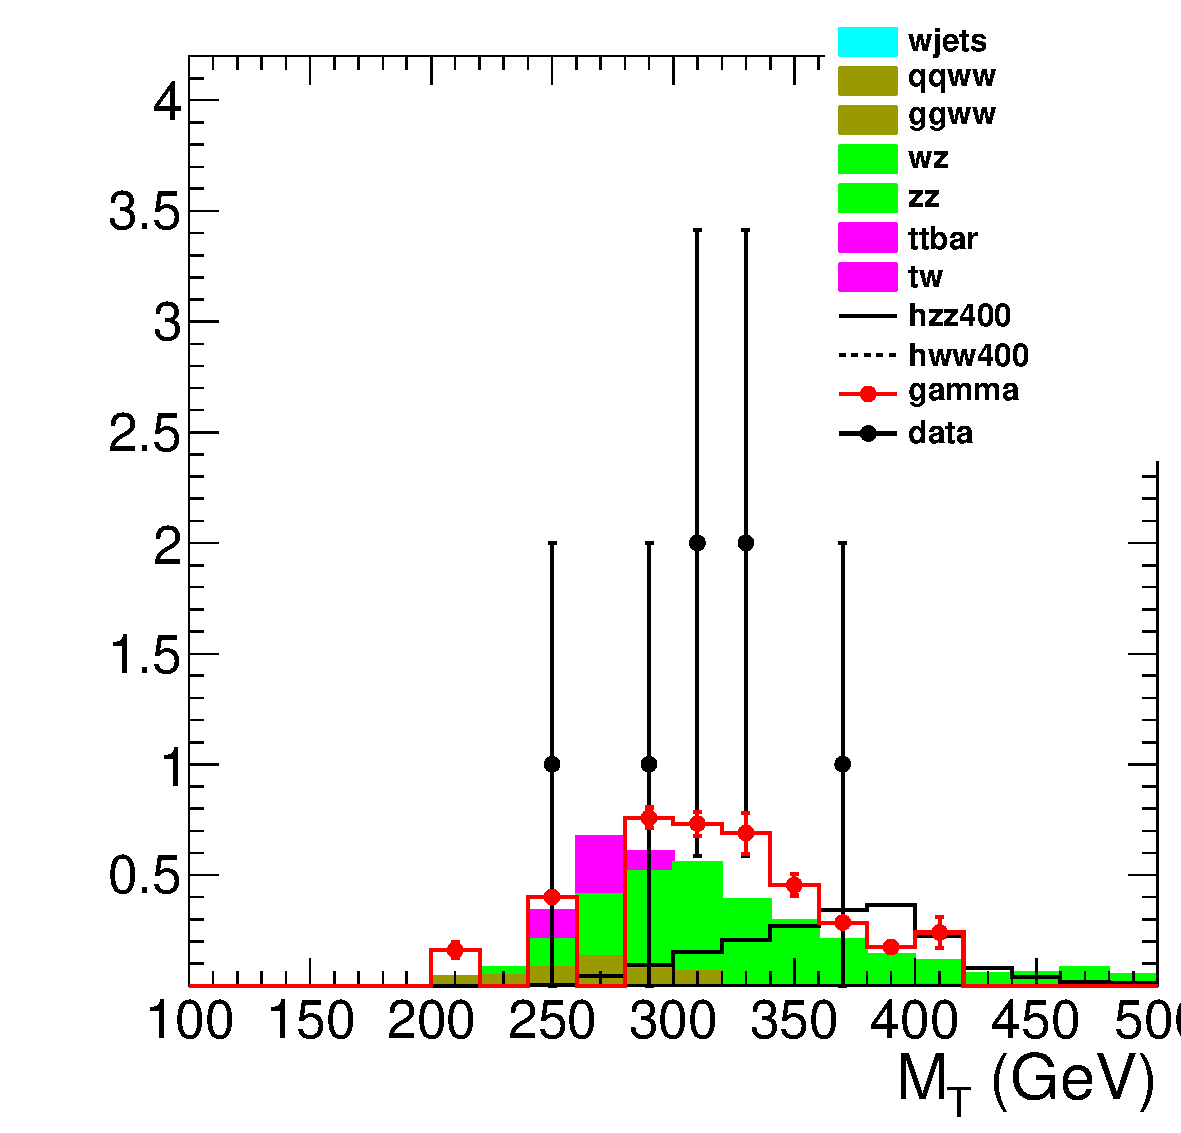
\includegraphics[width=.3\textwidth]{figures/hzz400_mt_1j.pdf}}
\caption{Transverse mass $m_T$ distribution after the full $\hzz$ ($m_H = 400\GeVcc$) selection observed in
data corresponding to $1092\pm7$~\ipb data in 0-Jet~\subref{subfig:mt_0j} and 1-Jet~\subref{subfig:mt_1j}
bins compared to the expected from simulation for signal and background. 
The MC backgrounds are scaled as appropriate and the photon+jets estimate of the Z+jets background is added to the stack.}
\end{center}
\end{figure}
%%%%%%%%

